% H2 Mathematics (9758) Paper 2 suggested solutions — O/N 2026
% Fonts: prelim_fonts (Times New Roman + TeX Gyre Termes Math)
\documentclass[a4paper,11pt,oneside]{article}
\usepackage{geometry}
\geometry{a4paper, top=20mm, bottom=22mm, left=20mm, right=20mm, headsep=6mm, footskip=12mm}
\usepackage{fontspec}
\usepackage{unicode-math}
% =====================================================================
% prelim_fonts.tex: fonts of the real 9758 prelim papers (Word + MathType; pdffonts on
% ACJC 2026 P1/P2, ACJC 2025 P1, JPJC 2026, RVHS 2026, CJC/DHS/TJC/NYJC/HCI/EJC 2025):
%   text Times New Roman; cover/footer Arial; RI page footer Calibri (here Carlito);
%   maths = MathType: Times New Roman letters/digits (italic variables; upright digits,
%   function names, d, e, f), SymbolMT for the integral, sigma, pi and = + < >,
%   scripts 7 pt on 12 pt (about 58 %), tight operator spacing.
% Candidate C (teacher-approved 13 Oct 2026): the real Times New Roman and Arial
% (ttf-mscorefonts-installer) + URW Standard Symbols PS (fonts-urw-base35, a SymbolMT
% clone with the same Symbol encoding) for the integral, sigma, pi, = + < >;
% TeX Gyre Termes Math only for what MathType draws itself (radicals, stretchy brackets,
% fraction bars, arrows). House style: upright d (\mathrm{d}x), upright e and f.
% Loaded once by di_style / de_core (HW sheets) and prelim_style (Tests, solutions).
% =====================================================================
\ifdefined\prelimfontsloaded\endinput\fi
\def\prelimfontsloaded{1}
\edef\pfrestoreat{\catcode`\noexpand\@=\the\catcode`\@\relax}\makeatletter
% MathType script sizes: 7 pt superscripts on 12 pt text (58 %), 5 pt second level
\DeclareMathSizes{12}{12}{7}{5}
\DeclareMathSizes{11}{11}{6.5}{5}
\DeclareMathSizes{10.95}{10.95}{6.5}{5}
\DeclareMathSizes{10}{10}{6}{5}
\DeclareMathSizes{9}{9}{5.5}{5}
\DeclareMathSizes{14.4}{14.4}{8.5}{6}
\setmainfont{Times New Roman}
\setsansfont{Arial}
\newfontfamily\coverfont{Arial}
\newfontfamily\calibrifont{Carlito}
\usepackage{unicode-math}
\setmathfont{TeX Gyre Termes Math}
\setmathfont[range={up/{latin,Latin,num}}]{Times New Roman}
\setmathfont[range={it/{latin,Latin}}]{Times New Roman Italic}
\setmathfont[range={bfup/{latin,Latin,num}}]{Times New Roman Bold}
\setmathfont[range={"002B,"003D,"003C,"003E}]{Standard Symbols PS}
\newfontfamily\pf@sym{Standard Symbols PS}
\newfontfamily\pf@symi[FakeSlant=0.21]{Standard Symbols PS}
% MathType-like spacing (tighter than TeX around = + -)
\AtBeginDocument{\thickmuskip=2.5mu plus 1mu\medmuskip=1.5mu plus 1mu\thinmuskip=3mu
% Symbol integral and sigma (18 pt at 12 pt text, as MathType), slanted Symbol pi
 \renewcommand{\int}{\mathop{\vcenter{\hbox{\pf@sym\fontsize{\fpeval{1.5*\f@size}}{0pt}\selectfont\char"F2}}}\nolimits}%
 \renewcommand{\sum}{\mathop{\vcenter{\hbox{\pf@sym\fontsize{\fpeval{1.5*\f@size}}{0pt}\selectfont\char"E5}}}\limits}%
 \renewcommand{\pi}{\mathord{\text{\pf@symi\char"70}}}}
\pfrestoreat

\usepackage{amsmath}
\usepackage{fancyhdr}
\usepackage{enumitem}
\usepackage{tcolorbox}
\tcbuselibrary{breakable,skins}
\usepackage{tikz}
\usetikzlibrary{arrows.meta,calc,patterns}
\usepackage{pgfplots}
\pgfplotsset{compat=1.18}
\usepackage{booktabs}
\usepackage{array}
\usepackage{setspace}
\usepackage{needspace}
\usepackage{xcolor}
\setlength{\parindent}{0pt}
\setlength{\parskip}{0.7ex}
\linespread{1.15}
\pagestyle{fancy}
\fancyhf{}
\lhead{\small H2 Mathematics (9758) Paper 2 suggested solutions}
\rhead{\small Compiled by Maximus Pung Jun}
\cfoot{\small\thepage}
\renewcommand{\headrulewidth}{0.4pt}

% Solution box (question then solution box)
\newtcolorbox{solbox}{
  enhanced, breakable,
  colback=white, colframe=black!70,
  boxrule=0.6pt, sharp corners,
  left=3mm, right=3mm, top=2mm, bottom=2mm,
  before skip=1.5mm, after skip=5mm,
  title={Solution}, fonttitle=\bfseries\small,
  coltitle=black, colbacktitle=black!8,
  toptitle=1mm, bottomtitle=1mm
}

% Question heading
\newcommand{\Qhead}[1]{\par\needspace{14\baselineskip}\medskip\noindent{\large\bfseries #1}\par\smallskip}
\newcommand{\partlabel}[1]{\par\needspace{3\baselineskip}\smallskip\noindent\textbf{#1}\quad}
\newcommand{\ans}[1]{\par\smallskip\noindent\textbf{Answer:}\ #1\par}
\newcommand{\mk}[1]{\hfill[#1]}

% upright d
\newcommand{\dx}{\,\mathrm{d}x}
\newcommand{\ii}{\mathbf{i}}
\newcommand{\jj}{\mathbf{j}}
\newcommand{\kk}{\mathbf{k}}
\newcommand{\vect}[1]{\mathbf{#1}}

\begin{document}
\thispagestyle{fancy}
\begin{center}
{\LARGE\bfseries H2 Mathematics (9758) Paper 2 suggested solutions}\\[1.2ex]
{\large Compiled by Maximus Pung Jun}\\[0.8ex]
{\normalsize October/November 2026 \quad 9758/02}
\end{center}
\vspace{1.5ex}
\noindent\rule{\textwidth}{0.8pt}\par
\vspace{1.2ex}
\noindent{\small\textit{Disclaimer: I am not responsible for any wrong answers. These are just suggested solutions.}}\par
\vspace{1.2ex}
\noindent\rule{\textwidth}{0.8pt}\par
\vspace{2ex}


\clearpage
\thispagestyle{fancy}
\noindent{\large\bfseries Final answers}\par
\vspace{0.2ex}
\noindent{\small Section A: Pure Mathematics}\par
\vspace{0.1ex}
\begin{itemize}[leftmargin=2.0em,itemsep=0.02ex,topsep=0.05ex,parsep=0pt]
\item[\textbf{1}] $\begin{pmatrix}-2/3\\2/3\\1/3\end{pmatrix}$ or $\begin{pmatrix}2/3\\-2/3\\-1/3\end{pmatrix}$
\item[\textbf{2(a)(i)}] $V=\dfrac{1}{3}\pi k^{2}h^3$
\item[\textbf{2(a)(ii)}] Shown
\item[\textbf{2(b)}] $y=\dfrac{1}{5}$ or $y=\dfrac{9}{5}$
\item[\textbf{3(a)}] Roots $1-2\mathrm{i}$, $-3$;\ $p=1$,\ $q=15$
\item[\textbf{3(b)(i)}] $\overrightarrow{OC}=\overrightarrow{BA}$, $\overrightarrow{OD}=\overrightarrow{AB}$; reflections through $O$
\item[\textbf{3(b)(ii)}] Reflection in the real axis
\item[\textbf{4(a)}] $r=2$,\ $d=3a$,\ $a\in\mathbb{R}\setminus\{0\}$
\item[\textbf{4(b)}] $n=11$
\item[\textbf{5(a)}] $(0,0)$, $\bigl(\tfrac{\pi}{2},0\bigr)$, $(\pi,0)$;\ see sketch
\item[\textbf{5(b)}] $\bigl(\tfrac{\pi}{6},\tfrac{3\sqrt{3}}{8}\bigr)$
\item[\textbf{5(c)}] $\dfrac{3}{8}$
\end{itemize}
\vspace{0.25ex}
\noindent{\small Section B: Probability and Statistics}\par
\vspace{0.1ex}
\begin{itemize}[leftmargin=2.0em,itemsep=0.02ex,topsep=0.05ex,parsep=0pt]
\item[\textbf{6(a)}] Sample
\item[\textbf{6(b)}] Equal chance / more representative / less bias
\item[\textbf{6(c)}] $557172$
\item[\textbf{7(a)}] $8$
\item[\textbf{7(b)(i)}] Shown ($P(A\cap B)=0.236\neq 0$)
\item[\textbf{7(b)(ii)}] Not independent
\item[\textbf{8(a)}] Draw a scatter diagram
\item[\textbf{8(b)(i)}] Little or no linear correlation
\item[\textbf{8(b)(ii)}] See sketch
\item[\textbf{8(c)(i)}] See sketch; not linear (levels off)
\item[\textbf{8(c)(ii)}] $y=c\sqrt{x}+d$ better
\item[\textbf{8(c)(iii)}] $17.9$ (3 s.f.)
\item[\textbf{9(a)}] $0.145$
\item[\textbf{9(b)}] $0.724$
\item[\textbf{9(c)}] $0.903$
\item[\textbf{9(d)}] $0.740$
\item[\textbf{9(e)}] $p=0.072$ or $0.400$
\item[\textbf{10(a)(i)}] $0.181$
\item[\textbf{10(a)(ii)}] $0.531$
\item[\textbf{10(a)(iii)}] $0.274$
\item[\textbf{10(b)}] $0.338$
\item[\textbf{11(a)(i)}] $\mathrm{H}_0:\mu=400$,\ $\mathrm{H}_1:\mu\neq 400$
\item[\textbf{11(a)(ii)}] $\bar{x}\le 398.1$ or $\bar{x}\ge 401.9$
\item[\textbf{11(a)(iii)}] Reject $\mathrm{H}_0$; mean no longer $400$ g
\item[\textbf{11(b)(i)}] Testing whether mean mass $>500$ g
\item[\textbf{11(b)(ii)}] $1.645$ (or $1.65$)
\item[\textbf{11(b)(iii)}] Non-random sample; small $n$ with no normality assumption
\end{itemize}
\clearpage
\noindent\textbf{Section A: Pure Mathematics [40 marks]}
\Qhead{1}
Find a unit vector that is perpendicular to both $3\ii - 2\jj + 10\kk$ and $2\ii + 3\jj - 2\kk$.\mk{4}

\begin{solbox}
\begin{align*}
\begin{pmatrix}3\\-2\\10\end{pmatrix}\times\begin{pmatrix}2\\3\\-2\end{pmatrix}
&= \begin{pmatrix}
(-2)(-2)-(10)(3)\\[0.4ex]
(10)(2)-(3)(-2)\\[0.4ex]
(3)(3)-(-2)(2)
\end{pmatrix}\\
&= \begin{pmatrix}4-30\\[0.4ex]20+6\\[0.4ex]9+4\end{pmatrix}
= \begin{pmatrix}-26\\26\\13\end{pmatrix}
\end{align*}
\begin{align*}
\left|\begin{pmatrix}-26\\26\\13\end{pmatrix}\right|
&= \sqrt{(-26)^2 + 26^2 + 13^2}\\
&= \sqrt{676 + 676 + 169}\\
&= \sqrt{1521}\\
&= 39
\end{align*}
\begin{align*}
\text{unit vector}
&= \dfrac{1}{39}\begin{pmatrix}-26\\26\\13\end{pmatrix}
= \begin{pmatrix}-2/3\\[0.3ex]2/3\\[0.3ex]1/3\end{pmatrix}
\end{align*}
(Alternatively $\begin{pmatrix}2/3\\[0.3ex]-2/3\\[0.3ex]-1/3\end{pmatrix}$.)
\end{solbox}
\clearpage
\Qhead{2}
\partlabel{(a)(i)}
Use calculus to find the volume generated when the line $y=kx$, for $0\le x\le h$, is rotated through $2\pi$ radians about the $x$-axis.\mk{3}
\partlabel{(ii)}
Hence show that the volume of a cone of height $h$ and base radius $r$ is $\dfrac{1}{3}\pi r^2h$.\mk{1}
\partlabel{(b)}
The straight line $y=kx$ cuts the curve $(x-k)^2+y^2=k^2$ at the point where $x=0.6$. Find exactly the possible values of $y$ at this point.\mk{3}

\begin{solbox}
\partlabel{(a)(i)}
\begin{align*}
V&=\int_0^h\pi y^2\dx\\
&=\pi k^2\int_0^h x^2\dx\\
&=\pi k^2\left[\dfrac{x^3}{3}\right]_0^h\\
&=\dfrac{1}{3}\pi k^2h^3.
\end{align*}
\partlabel{(a)(ii)}
\begin{center}
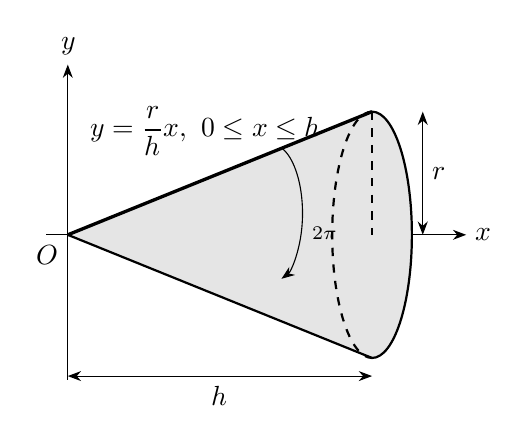
\begin{tikzpicture}[scale=0.92,>=Stealth]
  % axes
  \draw[->] (-0.3,0) -- (5.5,0) node[right]{$x$};
  \draw[->] (0,-2.0) -- (0,2.35) node[above]{$y$};
  \node[below left] at (0,0) {$O$};
  % shaded right circular cone (rotation of the line about the x-axis)
  \fill[black!10]
    (0,0) -- (4.2,1.7)
    arc[start angle=90, end angle=-90, x radius=0.55, y radius=1.7]
    -- cycle;
  % base ellipse
  \draw[thick] (4.2,1.7) arc[start angle=90, end angle=-90, x radius=0.55, y radius=1.7];
  \draw[thick,dashed] (4.2,1.7) arc[start angle=90, end angle=270, x radius=0.55, y radius=1.7];
  % lower generator
  \draw[thick] (0,0) -- (4.2,-1.7);
  % original line y=(r/h)x
  \draw[very thick] (0,0) -- (4.2,1.7);
  \node[above] at (1.9,0.95) {$y=\dfrac{r}{h}x,\ 0\le x\le h$};
  % radius mark at x=h
  \draw[dashed] (4.2,1.7) -- (4.2,0);
  \draw[<->] (0,-1.95) -- (4.2,-1.95) node[midway,below]{$h$};
  \draw[<->] (4.9,0) -- (4.9,1.7) node[midway,right]{$r$};
  % rotation about x-axis
  \draw[->] (2.95,1.2) arc[start angle=72, end angle=-72, x radius=0.42, y radius=0.95];
  \node[font=\scriptsize] at (3.55,0.02) {$2\pi$};
\end{tikzpicture}
\end{center}
\begin{align*}
r&=kh\quad\Rightarrow\quad k=\dfrac{r}{h}\\
V&=\dfrac{1}{3}\pi\left(\dfrac{r}{h}\right)^2h^3
=\dfrac{1}{3}\pi r^2h.
\end{align*}
\partlabel{(b)}
At $x=\dfrac{3}{5}$, $y=k\cdot\dfrac{3}{5}$:
\begin{align*}
\left(\dfrac{3}{5}-k\right)^2 + \left(\dfrac{3k}{5}\right)^2 &= k^2\\
\dfrac{9}{25} - \dfrac{6k}{5} + k^2 + \dfrac{9k^2}{25} &= k^2\\
\dfrac{9}{25} - \dfrac{6k}{5} + \dfrac{9k^2}{25} &= 0\\
9 - 30k + 9k^2 &= 0\\
9k^2 - 30k + 9 &= 0\\
3k^2 - 10k + 3 &= 0\\
(3k-1)(k-3) &= 0\\
k &= \dfrac{1}{3}\quad\text{or}\quad k=3
\end{align*}
\begin{align*}
y &= \dfrac{1}{3}\cdot\dfrac{3}{5} = \dfrac{1}{5}
\qquad\text{or}\qquad
y = 3\cdot\dfrac{3}{5} = \dfrac{9}{5}
\end{align*}
\end{solbox}
\clearpage
\Qhead{3}
\partlabel{(a)}
One of the roots of the equation $z^3+pz^2-z+q=0$, where $p$ and $q$ are real numbers, is $1+2\mathrm{i}$.

Find the other roots of the equation, the value of $p$ and the value of $q$.\mk{5}
\partlabel{(b)}
The points $A$ and $B$ on the Argand diagram represent the complex numbers $w_1$ and $w_2$ respectively.
\begin{center}
\begin{tikzpicture}[scale=.7,>=Stealth]
\draw[->] (-4.6,0)--(3,0) node[right]{Re};
\draw[->] (0,-2.2)--(0,2.8) node[above]{Im};
\node[below left] at (0,0){$O$};
\node at (-3,1){$\times$}; \node[above left] at (-3,1){$A$};
\node at (1,-1){$\times$}; \node[below right] at (1,-1){$B$};
\end{tikzpicture}
\end{center}
The complex number $w_3$ is defined as $w_3=w_1-w_2$, and the complex number $w_4$ is defined as $w_4=w_2-w_1$.
\partlabel{(i)}
On the copy of the Argand diagram in the Printed Answer Booklet, mark the point $C$ that represents $w_3$ and the point $D$ that represents $w_4$.

State the geometrical relationship between points $C$ and $D$.\mk{3}

The points $E$ and $F$ represent the complex numbers $w_1^*$ and $w_2^*$ respectively.
\partlabel{(ii)}
Describe the transformation that maps the line $AB$ onto the line $EF$.\mk{2}

\begin{solbox}
\partlabel{(a)}
Since $p$ and $q$ are real, $1-2\mathrm{i}$ is also a root.
Let the third root be $\alpha$. Then
\begin{align*}
\bigl(z-(1+2\mathrm{i})\bigr)\bigl(z-(1-2\mathrm{i})\bigr)(z-\alpha) &= 0\\
\bigl(z^2 - 2z + 5\bigr)(z-\alpha) &= 0\\
z^3 - (\alpha+2)z^2 + (5+2\alpha)z - 5\alpha &= 0
\end{align*}
Comparing with $z^3 + pz^2 - z + q = 0$:
\begin{align*}
5 + 2\alpha &= -1\\
2\alpha &= -6\\
\alpha &= -3
\end{align*}
\begin{align*}
p &= -(\alpha+2) = -(-3+2) = 1\\
q &= -5\alpha = -5(-3) = 15
\end{align*}
The other roots are $1-2\mathrm{i}$ and $-3$, with $p=1$ and $q=15$.
\partlabel{(b)(i)}
\begin{align*}
\overrightarrow{OC}&=\overrightarrow{BA},&\quad w_3&=w_1-w_2,\\
\overrightarrow{OD}&=\overrightarrow{AB},&\quad w_4&=-w_3.
\end{align*}
\begin{center}
\begin{tikzpicture}[scale=.75,>=Stealth]
\draw[->] (-5,0)--(5,0) node[right]{Re};
\draw[->] (0,-2.8)--(0,3) node[above]{Im};
\node[below left] at (0,0){$O$};
\fill (-3,1) circle (2pt) node[above left]{$A$};
\fill (1,-1) circle (2pt) node[below right]{$B$};
\fill (-4,2) circle (2pt) node[above left]{$C$};
\fill (4,-2) circle (2pt) node[below right]{$D$};
\draw[->,thick] (1,-1)--(-3,1);
\draw[->,thick] (0,0)--(-4,2);
\draw[->,thick] (0,0)--(4,-2);
\end{tikzpicture}
\end{center}
$C$ and $D$ are reflections of each other in the origin; $O$ is the midpoint of $CD$.
\partlabel{(b)(ii)}
The transformation is a reflection in the real axis.
\end{solbox}
\clearpage
\Qhead{4}
An arithmetic series has first term $a$ and common difference $d$, where $a\neq 0$ and $d\neq 0$. A geometric series has first term $a$ and common ratio $r$, where $r>0$.

The 6th term of the arithmetic series is equal to the 5th term of the geometric series.
The 22nd term of the arithmetic series is equal to the 7th term of the geometric series.

\partlabel{(a)}
Find the value of $r$ and an expression for $d$ in terms of $a$. Describe the set of possible values of $a$.\mk{5}



\partlabel{(b)}
The sum of the arithmetic series to 37 terms differs by $12a$ from the sum of the geometric series to $n$ terms. Find the value of $n$.\mk{4}

\begin{solbox}
\partlabel{(a)}
\begin{align*}
a + 5d &= ar^4\\
a + 21d &= ar^6
\end{align*}
Make $d$ the subject:
\begin{align*}
5d &= ar^4 - a = a(r^4 - 1)\\
d &= \dfrac{a(r^4 - 1)}{5}
\end{align*}
\begin{align*}
21d &= ar^6 - a = a(r^6 - 1)\\
d &= \dfrac{a(r^6 - 1)}{21}
\end{align*}
Equate the two expressions for $d$:
\begin{align*}
\dfrac{a(r^4 - 1)}{5} &= \dfrac{a(r^6 - 1)}{21}
\end{align*}
Since $a\neq 0$,
\begin{align*}
21(r^4 - 1) &= 5(r^6 - 1)\\
21r^4 - 21 &= 5r^6 - 5\\
0 &= 5r^6 - 21r^4 + 16
\end{align*}
Let $u=r^2$ ($u>0$):
\begin{align*}
5u^3 - 21u^2 + 16 &= 0\\
(u-1)(u-4)(5u+4) &= 0\\
u &= 1\quad\text{or}\quad u=4
\end{align*}
If $u=1$, then $r=1$ and $d=\dfrac{a(1-1)}{5}=0$, which is not allowed.

If $u=4$, then $r=2$ (since $r>0$) and
\begin{align*}
d &= \dfrac{a(2^4 - 1)}{5} = \dfrac{15a}{5} = 3a
\end{align*}
Since $d\neq 0$, we need $a\neq 0$.

Thus $r=2$, $d=3a$, and $a\in\mathbb{R}\setminus\{0\}$.
\partlabel{(b)}
\begin{align*}
S_{37}
&= \dfrac{37}{2}\bigl(2a + 36\cdot 3a\bigr)\\
&= \dfrac{37}{2}(2a + 108a)\\
&= \dfrac{37}{2}\cdot 110a\\
&= 2035a
\end{align*}
\begin{align*}
S_n &= a\dfrac{2^n - 1}{2-1} = a(2^n - 1)
\end{align*}
\begin{align*}
\bigl|S_{37} - S_n\bigr| &= 12|a|\\
\bigl|2035a - a(2^n - 1)\bigr| &= 12|a|\\
\bigl|2035 - (2^n - 1)\bigr| &= 12
\qquad (a\neq 0)\\
\bigl|2036 - 2^n\bigr| &= 12
\end{align*}
From GC table (values of $\bigl|2036-2^n\bigr|$):
\begin{center}
\begin{tabular}{c|cccc}
$n$ & $10$ & $11$ & $12$ & $13$ \\
\hline
$2^n$ & $1024$ & $2048$ & $4096$ & $8192$ \\
$\bigl|2036-2^n\bigr|$ & $1012$ & $12$ & $2060$ & $6156$
\end{tabular}
\end{center}
When $n=11$, $\bigl|2036-2^{11}\bigr|=12$.

Hence $n=11$.
\end{solbox}
\clearpage
\Qhead{5}
\partlabel{(a)}
Sketch the graph of the curve $y = \cos^2 x\sin 2x$ for $0\le x\le\pi$, giving the exact coordinates of the points of intersection with the $x$-axis.\mk{2}



\partlabel{(b)}
Find the exact coordinates of the maximum point. You do not have to show this is a maximum point.\mk{4}



\partlabel{(c)}
Do not use a calculator in answering this part.
Find the exact area bounded by the curve, the $x$-axis and the lines $x=0$ and $x=\dfrac{1}{4}\pi$.\mk{4}





\begin{solbox}
\partlabel{(a)}
\begin{align*}
y &= \cos^2 x\cdot 2\sin x\cos x = 2\cos^3 x\sin x
\end{align*}
$y=0$ when $\cos x = 0$ or $\sin x = 0$:
\begin{align*}
x &= 0,\ \dfrac{\pi}{2},\ \pi
\end{align*}
Intercepts: $\bigl(0,0\bigr)$, $\bigl(\dfrac{\pi}{2},0\bigr)$, $\bigl(\pi,0\bigr)$.
\begin{center}
\begin{tikzpicture}
\begin{axis}[
  width=11cm, height=5.2cm,
  axis lines=middle,
  xlabel={$x$}, ylabel={$y$},
  xmin=-0.2, xmax=3.5, ymin=-1.1, ymax=1.1,
  xtick={0,0.5236,1.5708,2.618,3.1416},
  xticklabels={$0$, $\frac{\pi}{6}$, $\frac{\pi}{2}$, $\frac{5\pi}{6}$, $\pi$},
  ytick={-0.6495,0.6495},
  yticklabels={$-\frac{3\sqrt{3}}{8}$, $\frac{3\sqrt{3}}{8}$},
  samples=200, clip=false, trig format plots=rad
]
\addplot[thick, domain=0:pi, black] {2*(cos(x))^3*sin(x)};
\fill (0,0) circle (1.5pt);
\fill ({pi/2},0) circle (1.5pt);
\fill ({pi},0) circle (1.5pt);
\fill ({pi/6},{3*sqrt(3)/8}) circle (1.5pt);
\fill ({5*pi/6},{-3*sqrt(3)/8}) circle (1.5pt);
\end{axis}
\end{tikzpicture}
\end{center}
\partlabel{(b)}
\begin{align*}
\dfrac{\mathrm{d}y}{\mathrm{d}x}
&= 2\bigl(-3\cos^2 x\sin x\cdot\sin x + \cos^3 x\cos x\bigr)\\
&= 2\cos^2 x\bigl(-3\sin^2 x + \cos^2 x\bigr)
\end{align*}
Set $\dfrac{\mathrm{d}y}{\mathrm{d}x}=0$:
\begin{align*}
\cos^2 x = 0 &\quad\Rightarrow\quad x = \dfrac{\pi}{2}
\quad\text{(gives $y=0$)}\\[1mm]
\cos^2 x &= 3\sin^2 x\\
\cot^2 x &= 3\\
\tan^2 x &= \dfrac{1}{3}\\
\tan x &= \pm\dfrac{1}{\sqrt{3}}
\end{align*}
For $0<x<\pi$: $x=\dfrac{\pi}{6}$ or $x=\dfrac{5\pi}{6}$.
\begin{align*}
y\left(\dfrac{\pi}{6}\right)
&= 2\cos^3\dfrac{\pi}{6}\sin\dfrac{\pi}{6}
= 2\left(\dfrac{\sqrt{3}}{2}\right)^3\left(\dfrac{1}{2}\right)
= 2\cdot\dfrac{3\sqrt{3}}{8}\cdot\dfrac{1}{2}
= \dfrac{3\sqrt{3}}{8}
\end{align*}
\begin{align*}
y\left(\dfrac{5\pi}{6}\right)
&= -\dfrac{3\sqrt{3}}{8}
\end{align*}
Maximum point: $\left(\dfrac{\pi}{6},\dfrac{3\sqrt{3}}{8}\right)$.
\partlabel{(c)}
\begin{align*}
\text{Area}
&= \int_{0}^{\pi/4} 2\cos^3 x\sin x\dx
\end{align*}
Let $u=\cos x$, so $\mathrm{d}u = -\sin x\dx$.

When $x=0$, $u=1$; when $x=\dfrac{\pi}{4}$, $u=\dfrac{\sqrt{2}}{2}$.
\begin{align*}
\text{Area}
&= \int_{1}^{\sqrt{2}/2} 2u^3(-1)\,\mathrm{d}u
= 2\int_{\sqrt{2}/2}^{1} u^3\,\mathrm{d}u\\
&= 2\left[\dfrac{1}{4}u^4\right]_{\sqrt{2}/2}^{1}
= \dfrac{1}{2}\left(1 - \left(\dfrac{\sqrt{2}}{2}\right)^4\right)\\
&= \dfrac{1}{2}\left(1 - \dfrac{4}{16}\right)
= \dfrac{1}{2}\left(1 - \dfrac{1}{4}\right)
= \dfrac{1}{2}\cdot\dfrac{3}{4}
= \dfrac{3}{8}
\end{align*}
\end{solbox}
\clearpage
\noindent\textbf{Section B: Probability and Statistics [60 marks]}
\Qhead{6}
The employees of a certain company are put into teams based on the jobs that they do. The company consists of 22 employees from the Red team, 18 from the Blue team, 9 from the Green team and 6 from the Yellow team.

The manager of the company wishes to find out the opinions of the employees about the office facilities provided for employees. Questionnaires are given to all employees but only the 40 employees from the Red team and the Blue team return them.

\partlabel{(a)}
Explain whether these 40 employees comprise a sample or a population.\mk{1}



The manager decides to form a committee of employees to discuss the results of the questionnaire.

\partlabel{(b)}
State an advantage of choosing a random sample of employees for the committee.\mk{1}



The manager decides that the committee will consist of 5 employees, such that
\begin{itemize}[leftmargin=1.8em,itemsep=0.3ex]
\item the committee includes an employee from the Green team,
\item at least three teams are represented on the committee and
\item there are more members from the Red team than from any other single team on the committee.
\end{itemize}

\partlabel{(c)}
Find the number of ways in which the committee can be formed.\mk{4}

\begin{solbox}
\partlabel{(a)}
They comprise a \textbf{sample}, because they are only a subset of all the employees of the company (the Green and Yellow teams did not return the questionnaires).
\partlabel{(b)}
Every employee has an equal chance of being chosen, so the committee is more likely to be representative / bias is reduced.
\partlabel{(c)}
Let the committee have $r$ members from Red. Since Red must have strictly more members than any other team and the total is 5 with at least one Green,
the possible compositions are:
\begin{align*}
&(2\text{ Red},\ 1\text{ Blue},\ 1\text{ Green},\ 1\text{ Yellow})\\
&(3\text{ Red},\ 1\text{ Blue},\ 1\text{ Green},\ 0\text{ Yellow})\\
&(3\text{ Red},\ 0\text{ Blue},\ 1\text{ Green},\ 1\text{ Yellow})
\end{align*}
\begin{align*}
\text{Number of ways}
&= \binom{22}{2}\binom{18}{1}\binom{9}{1}\binom{6}{1}
+ \binom{22}{3}\binom{18}{1}\binom{9}{1}
+ \binom{22}{3}\binom{9}{1}\binom{6}{1}\\
&= 231\cdot 18\cdot 9\cdot 6
+ 1540\cdot 18\cdot 9
+ 1540\cdot 9\cdot 6\\
&= 224532 + 249480 + 83160\\
&= 557172
\end{align*}
\end{solbox}
\clearpage
\Qhead{7}
\partlabel{(a)}
A bag contains 20 balls. Some of the balls are red, some are yellow and the rest are blue. Two balls are taken, at random and at the same time, from the bag. The probability that one of the balls is red and the other one is yellow is $\dfrac{28}{95}$. The probability that one of the balls is red and the other one is blue is $\dfrac{4}{19}$. Determine the number of red balls originally in the bag.\mk{5}



\partlabel{(b)}
Events $A$ and $B$ are such that $P(A\cap B')=0.364$, $P(A'\cap B)=0.124$ and $P((A\cup B)')=0.276$.

\partlabel{(i)}
Show that $A$ and $B$ are not mutually exclusive events.\mk{2}



\partlabel{(ii)}
Determine whether $A$ and $B$ are independent events.\mk{2}

\begin{solbox}
\partlabel{(a)}
Let there be $R$ red, $Y$ yellow and $B$ blue balls, so $R+Y+B=20$.
\begin{align*}
\dfrac{\binom{R}{1}\binom{Y}{1}}{\binom{20}{2}} &= \dfrac{28}{95}\\
\dfrac{RY}{190} &= \dfrac{28}{95}\\
RY &= 56
\end{align*}
\begin{align*}
\dfrac{RB}{190} &= \dfrac{4}{19}\\
RB &= 40
\end{align*}
\begin{align*}
Y + B &= 20 - R\\
\dfrac{56}{R} + \dfrac{40}{R} &= 20 - R\\
\dfrac{96}{R} &= 20 - R\\
96 &= 20R - R^2\\
R^2 - 20R + 96 &= 0\\
(R-8)(R-12) &= 0\\
R &= 8\quad\text{or}\quad R=12
\end{align*}
If $R=12$, then $Y=\dfrac{56}{12}$ is not an integer.

If $R=8$, then $Y=7$ and $B=5$, which are positive integers.

Hence there are $8$ red balls originally in the bag.
\partlabel{(b)(i)}
\begin{align*}
P(A\cup B) &= 1 - P((A\cup B)') = 1 - 0.276 = 0.724
\end{align*}
\begin{align*}
P(A\cup B) &= P(A\cap B') + P(A'\cap B) + P(A\cap B)\\
0.724 &= 0.364 + 0.124 + P(A\cap B)\\
P(A\cap B) &= 0.236 \neq 0
\end{align*}
Hence $A$ and $B$ are not mutually exclusive.
\partlabel{(b)(ii)}
\begin{align*}
P(A) &= P(A\cap B') + P(A\cap B) = 0.364 + 0.236 = 0.600\\
P(B) &= P(A'\cap B) + P(A\cap B) = 0.124 + 0.236 = 0.360
\end{align*}
\begin{align*}
P(A)P(B) &= 0.600\times 0.360 = 0.216\\
P(A\cap B) &= 0.236 \neq 0.216
\end{align*}
Hence $A$ and $B$ are not independent.
\end{solbox}
\clearpage
\Qhead{8}
Three researchers are investigating the effect of the amount of fertiliser used on crop yields.

\partlabel{(a)}
Tang uses Fertiliser A. He calculates that the product moment correlation coefficient between the amount of fertiliser used per square metre and the crop yield per square metre is $0.98$.
State what else Tang should do before deciding whether a linear model is a good fit to the data.\mk{1}



\partlabel{(b)}
Xi uses Fertiliser B. He finds that the product moment correlation coefficient between the amount of fertiliser used per square metre and the crop yield per square metre is approximately $0$.

\partlabel{(i)}
Explain how Xi should interpret the results of his investigation.\mk{1}



\partlabel{(ii)}
Sketch a scatter diagram with at least 5 points to illustrate a product moment correlation coefficient of approximately $0$.\mk{1}



\partlabel{(c)}
Leia uses Fertiliser C. She sets up 6 test plots of land. The table shows the amount of fertiliser, $x$ grams, used per square metre of each plot and the crop yield, $y$ kilograms, per square metre of each plot.

\begin{center}
\begin{tabular}{c|cccccc}
$x$ & 0 & 5 & 10 & 15 & 20 & 25 \\
\hline
$y$ & 7 & 14 & 16 & 21 & 21 & 20
\end{tabular}
\end{center}

\partlabel{(i)}
Sketch the scatter diagram for Leia's data, and explain how you know that the crop yield is not linearly related to the amount of fertiliser used.\mk{2}



\partlabel{(ii)}
By drawing sketches of the equations below, where $c,d,e$ and $f$ are positive constants, explain which is a better model for the relationship between the amount of fertiliser used and the crop yield.
\[ y = c\sqrt{x} + d \qquad\qquad y = ex^2 + f \]
\mk{3}



\partlabel{(iii)}
Use the better model to find an estimate for the crop yield per square metre when the amount of fertiliser used is 13 grams per square metre. Give your answer correct to 3 significant figures.\mk{3}

\begin{solbox}
\partlabel{(a)}
He should draw a scatter diagram (to check that the relationship is approximately linear / that there are no outliers).
\partlabel{(b)(i)}
There is little or no linear correlation between the amount of fertiliser used and the crop yield (there may still be a non-linear relationship).
\partlabel{(b)(ii)}
\begin{center}
\begin{tikzpicture}[scale=0.7]
  \draw[->] (0,0) -- (6.2,0) node[right]{\small fertiliser};
  \draw[->] (0,0) -- (0,4.2) node[above]{\small yield};
  \foreach \p in {(1,2.2),(1.8,3.1),(2.6,1.4),(3.5,2.8),(4.2,1.7),(5.1,3.0)} {
    \fill \p circle (2pt);
  }
\end{tikzpicture}
\end{center}
(Points form a random cloud with no linear trend.)
\partlabel{(c)(i)}
\begin{center}
\begin{tikzpicture}[scale=0.22]
  \draw[->] (0,0) -- (28,0) node[right]{\small $x$};
  \draw[->] (0,0) -- (0,24) node[above]{\small $y$};
  \foreach \x/\y in {0/7,5/14,10/16,15/21,20/21,25/20} {
    \fill (\x,\y) circle (8pt);
  }
  \node[below] at (0,0) {\scriptsize 0};
  \node[below] at (25,0) {\scriptsize 25};
  \node[left] at (0,7) {\scriptsize 7};
  \node[left] at (0,21) {\scriptsize 21};
\end{tikzpicture}
\end{center}
The points rise and then level off / fall slightly, so the relationship is not linear.
\partlabel{(c)(ii)}
\begin{center}
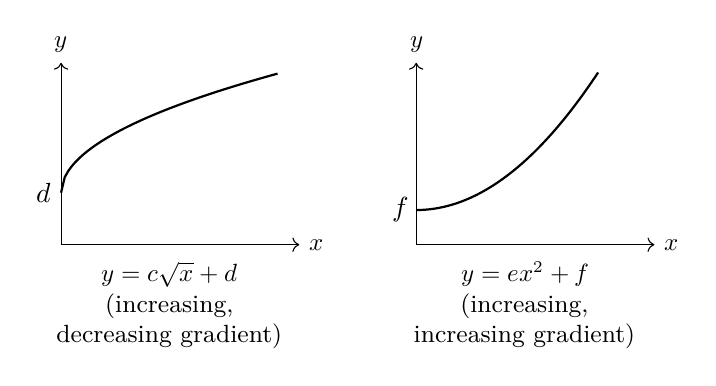
\begin{tikzpicture}[scale=0.55]
  \begin{scope}
    \draw[->] (0,0) -- (5.5,0) node[right]{\small $x$};
    \draw[->] (0,0) -- (0,4.2) node[above]{\small $y$};
    \draw[thick, domain=0:5, samples=60] plot (\x, {0.55*sqrt(5*\x)+1.2});
    \node[left] at (0,1.2){$d$};
    \node[align=center, font=\small] at (2.5,-1.4){$y=c\sqrt{x}+d$\\(increasing,\\decreasing gradient)};
  \end{scope}
  \begin{scope}[xshift=8.2cm]
    \draw[->] (0,0) -- (5.5,0) node[right]{\small $x$};
    \draw[->] (0,0) -- (0,4.2) node[above]{\small $y$};
    \draw[thick, domain=0:4.2, samples=60] plot (\x, {0.18*\x*\x+0.8});
    \node[left] at (0,0.8){$f$};
    \node[align=center, font=\small] at (2.5,-1.4){$y=ex^2+f$\\(increasing,\\increasing gradient)};
  \end{scope}
\end{tikzpicture}
\end{center}
The data increase then flatten, matching $y=c\sqrt{x}+d$ (decreasing gradient). The model $y=ex^2+f$ gets steeper, so $y=c\sqrt{x}+d$ is the better model.
\partlabel{(c)(iii)}
Using the model $y = c\sqrt{x} + d$ with least-squares regression on the data (GC):
\begin{align*}
c &\approx 2.91126, \qquad d \approx 7.40549
\end{align*}
\begin{align*}
y &= 2.91126\sqrt{13} + 7.40549 \approx 17.9
\end{align*}
(to 3 s.f.).
\end{solbox}
\clearpage
\Qhead{9}
Tringos are sweets that are made in four different colours: red, yellow, purple and green. They are sold in packets containing 12 randomly chosen sweets.

\partlabel{(a)}
A student wishes to estimate the proportion of Tringos that are green. She checks the contents of 100 randomly chosen packets of Tringos and finds the information summarised in the table.

\begin{center}
\begin{tabular}{c|ccccccc}
\shortstack{number of green sweets\\in a packet} & 0 & 1 & 2 & 3 & 4 & 5 & 6 or more \\
\hline
frequency & 15 & 32 & 27 & 18 & 6 & 2 & 0
\end{tabular}
\end{center}

Use the information in the table to estimate the probability that a randomly chosen Tringo is green.\mk{2}



The probability that a randomly chosen Tringo is red is $0.3$.

\partlabel{(b)}
Find the probability that a packet of 12 Tringos contains fewer than 5 red sweets.\mk{1}



\partlabel{(c)}
Find the probability that at least 4 out of 7 randomly chosen packets of Tringos contain fewer than 5 red sweets.\mk{2}



Tringos are delivered to shops in cartons containing 72 randomly chosen packets of 12 sweets.
\partlabel{(d)}
Find the probability that there are more than 250 red sweets in a randomly chosen carton of Tringos.\mk{2}



The probability that a randomly chosen Tringo is yellow is $p$.
\partlabel{(e)}
Given that the probability that a randomly chosen packet of 12 Tringos contains either 2 or 3 yellow sweets is $0.206$, find the two possible values of $p$. Give your values correct to 3 decimal places.\mk{3}

\begin{solbox}
\partlabel{(a)}
\begin{align*}
\text{Total number of green sweets}
&= 0\cdot 15 + 1\cdot 32 + 2\cdot 27 + 3\cdot 18 + 4\cdot 6 + 5\cdot 2 + 6\cdot 0\\
&= 174
\end{align*}
\begin{align*}
\text{Total number of sweets} &= 100\times 12 = 1200
\end{align*}
\begin{align*}
\text{Estimate of probability} &= \dfrac{174}{1200} = 0.145
\end{align*}
\partlabel{(b)}
Let $X\sim\mathrm{B}(12,0.3)$.
\begin{align*}
P(X\le 4) &= 0.724\quad\text{(3 s.f.)}\qquad\text{(by GC)}
\end{align*}
\partlabel{(c)}
Let $q = P(X\le 4) = 0.723655\ldots$ and let $Y\sim\mathrm{B}(7,q)$.
\begin{align*}
P(Y\ge 4) &= 0.903\quad\text{(3 s.f.)}\qquad\text{(by GC)}
\end{align*}
\partlabel{(d)}
Let $R$ be the number of red sweets in a carton.
\[
R\sim\mathrm{B}(72\times12,0.3)=\mathrm{B}(864,0.3).
\]
\begin{align*}
P(R>250)&=0.740\quad\text{(3 s.f.)}\qquad\text{(by GC)}
\end{align*}
\partlabel{(e)}
Let $W\sim\mathrm{B}(12,p)$.
\begin{align*}
P(W=2)+P(W=3) &= 0.206\\
\binom{12}{2}p^2(1-p)^{10} + \binom{12}{3}p^3(1-p)^9 &= 0.206
\end{align*}
From GC, $p = 0.072$ or $p = 0.400$ (to 3 d.p.).
\end{solbox}
\clearpage
\Qhead{10}
In this question you should assume that the distributions are all independent of each other.

Mrs Ng lives in Aytown. She often drives to the neighbouring towns of Beetown and Seatown.
\partlabel{(a)}
The time taken, in minutes, for Mrs Ng to drive from Aytown to Beetown using her usual route has the distribution $\mathrm{N}(22,3^2)$.
\partlabel{(i)}
Find the probability that Mrs Ng takes between 22.5 and 24 minutes for a randomly chosen journey from Aytown to Beetown.\mk{1}

Mrs Ng often visits the shops in Beetown. The time, in minutes, she spends at the shops has the distribution $\mathrm{N}(75,12^2)$. The time taken for the journey from Beetown to Aytown also has the distribution $\mathrm{N}(22,3^2)$.
\partlabel{(ii)}
Find the probability that a randomly chosen trip from Aytown to the shops at Beetown and back to Aytown by Mrs Ng takes less than 2 hours.\mk{3}

The time taken, in minutes, for Mrs Ng to drive from Aytown to Beetown using an alternative route has the distribution $\mathrm{N}(25,4^2)$.
\partlabel{(iii)}
Find the probability that a randomly chosen journey from Aytown to Beetown using the alternative route takes less time than a randomly chosen journey using Mrs Ng's usual route.\mk{3}
\partlabel{(b)}
The time taken, in minutes, for the journey from Aytown to Seatown is also normally distributed. The probability that a randomly chosen journey takes less than 55 minutes is $0.873$ and the probability that a randomly chosen journey takes more than 49 minutes is $0.471$.

Find the probability that a randomly chosen journey from Aytown to Seatown takes between 45 and 50 minutes.\mk{4}

\begin{solbox}
\partlabel{(a)(i)}
Let $X\sim\mathrm{N}(22,3^2)$.
\begin{align*}
P(22.5 < X < 24) &= 0.181\quad\text{(3 s.f.)}\qquad\text{(by GC)}
\end{align*}
\partlabel{(a)(ii)}
Let $T = X_1 + S + X_2$, where $X_1,X_2\sim\mathrm{N}(22,3^2)$ and $S\sim\mathrm{N}(75,12^2)$.
\begin{align*}
\mathrm{E}(T) &= 22 + 75 + 22 = 119\\
\mathrm{Var}(T) &= 9 + 144 + 9 = 162
\end{align*}
So $T\sim\mathrm{N}(119,162)$.
\begin{align*}
P(T < 120) &= 0.531\quad\text{(3 s.f.)}\qquad\text{(by GC)}
\end{align*}
\partlabel{(a)(iii)}
Let $A\sim\mathrm{N}(25,4^2)$ and $U\sim\mathrm{N}(22,3^2)$, and let $D = A - U$.
\begin{align*}
\mathrm{E}(D) &= 25 - 22 = 3\\
\mathrm{Var}(D) &= 16 + 9 = 25
\end{align*}
So $D\sim\mathrm{N}(3,5^2)$.
\begin{align*}
P(A < U) &= P(D < 0) = 0.274\quad\text{(3 s.f.)}\qquad\text{(by GC)}
\end{align*}
\partlabel{(b)}
Let $T\sim\mathrm{N}(\mu,\sigma^2)$ and $Z\sim\mathrm{N}(0,1)$.
\begin{align*}
P(T < 55) &= 0.873\\
\Rightarrow\quad P\!\left(Z < \dfrac{55-\mu}{\sigma}\right) &= 0.873\\
\Rightarrow\quad \dfrac{55-\mu}{\sigma} &= 1.1407
\end{align*}
\begin{align*}
P(T > 49) &= 0.471\\
\Rightarrow\quad P(T < 49) &= 0.529\\
\Rightarrow\quad P\!\left(Z < \dfrac{49-\mu}{\sigma}\right) &= 0.529\\
\Rightarrow\quad \dfrac{49-\mu}{\sigma} &= 0.07276
\end{align*}
\begin{align*}
55 - \mu &= 1.1407\sigma\\
49 - \mu &= 0.07276\sigma
\end{align*}
Subtracting,
\begin{align*}
6 &= 1.06794\sigma\\
\sigma &\approx 5.618\\
\mu &= 55 - 1.1407\times 5.618 \approx 48.59
\end{align*}
So $T\sim\mathrm{N}(48.59,\ 5.618^2)$ approximately.
\begin{align*}
P(45 < T < 50) &= 0.338\quad\text{(3 s.f.)}\qquad\text{(by GC)}
\end{align*}
\end{solbox}
\clearpage
\Qhead{11}
\partlabel{(a)}
A company uses a machine to pack bird seed into packets. Packets should contain a mean mass of 400 grams of seed. Following maintenance to the packing machine, the owner of the company wishes to check that packets still contain a mean mass of 400 grams of seed. He decides to carry out a hypothesis test at the $5\%$ level of significance.

The owner finds the masses, $x$ grams, of bird seed in a random sample of packets. Summary data is as follows.
\[ n=40 \qquad \sum(x-400)=120 \qquad \sum(x-400)^2=1902 \]
\partlabel{(i)}
Write down the hypotheses for the test, defining the parameter(s) you use.\mk{2}
\partlabel{(ii)}
Find the critical region for the test, giving your answer in grams correct to 1 decimal place.\mk{4}
\partlabel{(iii)}
State the conclusion of the test in the context of the question.\mk{2}
\partlabel{(b)}
The company also has a machine that fills bags with pet food. The mean mass of pet food is stated to be 500 grams per bag. Following comments from customers, the owner of the company decides to carry out a z-test using
\begin{align*}
\mathrm{H}_0&:\ \mu=500\\
\mathrm{H}_1&:\ \mu>500.
\end{align*}
\partlabel{(i)}
State what the owner is testing for.\mk{2}
\partlabel{(ii)}
State the critical z-value used for this test when it is carried out at the $5\%$ level of significance.\mk{1}

The machine is used each week from Monday to Friday. The owner decides to take the last 5 bags filled on Monday, Wednesday and Friday one week, to make up a sample of 15 bags for his test.
\partlabel{(iii)}
Give two reasons why the owner's sample is not suitable for this test.\mk{2}

\begin{solbox}
\partlabel{(a)(i)}
Let $\mu$ be the population mean mass (in grams) of a packet of bird seed after maintenance.
\begin{align*}
\mathrm{H}_0&: \mu = 400\\
\mathrm{H}_1&: \mu \neq 400
\end{align*}
\partlabel{(a)(ii)}
\begin{align*}
\bar{x} &= 400 + \dfrac{120}{40} = 403
\end{align*}
\begin{align*}
s^2
&= \dfrac{1}{n-1}\left(\sum(x-400)^2 - \dfrac{\bigl(\sum(x-400)\bigr)^2}{n}\right)\\
&= \dfrac{1}{39}\left(1902 - \dfrac{120^2}{40}\right)\\
&= \dfrac{1}{39}\bigl(1902 - 360\bigr)\\
&= \dfrac{1542}{39}\\
&= 39.538\ldots
\end{align*}
Under $\mathrm{H}_0$, by the Central Limit Theorem ($n=40$ is large),
\[
\bar{X}\;\sim\;\mathrm{N}\!\left(400,\dfrac{s^2}{40}\right)
\quad\text{approximately.}
\]
Conduct a 2-tailed test at the $5\%$ level of significance.
\begin{center}
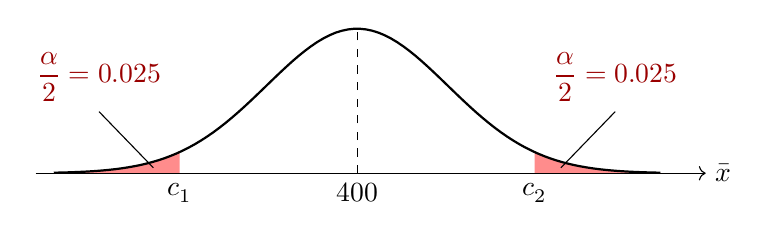
\begin{tikzpicture}[x=1.15cm,y=4.6cm]
\fill[red!45] (1.96,0) -- plot[domain=1.96:3.35,samples=40] (\x,{exp(-\x*\x/2)/sqrt(2*pi)}) -- (3.35,0) -- cycle;
\fill[red!45] (-3.35,0) -- plot[domain=-3.35:-1.96,samples=40] (\x,{exp(-\x*\x/2)/sqrt(2*pi)}) -- (-1.96,0) -- cycle;
\draw[->] (-3.55,0) -- (3.85,0) node[right]{$\bar{x}$};
\draw[thick] plot[domain=-3.35:3.35,samples=100] (\x,{exp(-\x*\x/2)/sqrt(2*pi)});
\draw[dashed] (0,0) -- (0,{1/sqrt(2*pi)});
\node[below] at (0,0){$400$};
\node[below] at (-1.96,0){$c_1$};
\node[below] at (1.96,0){$c_2$};
\draw (-2.25,0.015) -- (-2.85,0.17) node[above,red!60!black]{$\dfrac{\alpha}{2}=0.025$};
\draw (2.25,0.015) -- (2.85,0.17) node[above,red!60!black]{$\dfrac{\alpha}{2}=0.025$};
\end{tikzpicture}
\end{center}
By GC, $c_1 = 398.1$ and $c_2 = 401.9$ (to 1 d.p.).

Thus, critical region is $\bar{x}\le 398.1$ or $\bar{x}\ge 401.9$.
\partlabel{(a)(iii)}
Since $\bar{x}=403$ lies in the critical region, reject $\mathrm{H}_0$.

There is sufficient evidence at the $5\%$ level that the mean mass of a packet is no longer 400 grams.
\partlabel{(b)(i)}
The owner is testing whether the mean mass of a bag of pet food is greater than 500 grams.
\partlabel{(b)(ii)}
Critical $z$-value $= 1.645$ (or $1.65$).
\partlabel{(b)(iii)}
\begin{itemize}[leftmargin=1.8em,itemsep=0.4ex]
\item The sample is not random: only the last bags on three selected days are included, so it may be biased.
\item $n=15$ is small, and the population distribution of bag masses is not stated to be normal.
\end{itemize}
\end{solbox}
\vspace{3ex}
\begin{center}\textbf{END OF SUGGESTED SOLUTIONS}\end{center}
\end{document}
